%----------------------------------------------------------------------------
\chapter{Irodalmi áttekintés}
%----------------------------------------------------------------------------

\section{Mobil robotok irányítása}
A mobil robotok irányítása alapvető szerepet játszik az autonóm rendszerek hatékony működésében. Az autonóm mobil robotok  alkalmazási területeik két részre bonthatók, az egyik az olyan feladatok, amelyek nagy precizitást igényelnek és egy embernél gyorsabban, pontosabban szükségesek elvégezni, a másik a könnyen autómatizálható feladatok, ahol robotok alkalmazásával jelentős költségmegtakarítás érhető el. Például:

\begin{itemize}
    \item \textbf{Logisztika}: Raktári robotok optimalizálják az áruk szállítását, csökkentve az emberi erőforrás szükségletét és növelve a hatékonyságot.
    \item \textbf{Egészségügy}: Autonóm robotok biztosítják a steril környezetet és az időérzékeny anyagok szállítását kórházakban.
    \item \textbf{Mezőgazdaság}: Robotok segítenek a precíziós gazdálkodásban, például a növények állapotának monitorozásában vagy a gyomirtásban.
\end{itemize}

Az autonóm mobil robotok sikere nagyban függ a vezérlési rendszer minőségétől. Egy hatékony irányítórendszer:
\begin{enumerate}
    \item \textbf{Pontosan vezérli a robot mozgását} a megadott pályán.
    \item \textbf{Akadályokat kerül el biztonságosan}, az emberi és környezeti tényezőket figyelembe véve.
    \item \textbf{Döntéseket hoz valós időben} a változó környezetben.
    \item \textbf{Energiahatékony} működést biztosít, ami különösen fontos akkumulátorról működő rendszerek esetén.
\end{enumerate}

A mobil robotok irányítása különösen bonyolult, mivel figyelembe kell venni:
\begin{itemize}
    \item a robot kinematikai és dinamikai modelljét,
    \item a környezeti bizonytalanságokat, például dinamikus akadályokat,
    \item a rendszer korlátait, mint például a szenzorok pontosságát és a robot fizikáját.
\end{itemize}

\section{Robotok mechanikai felépítése}
Robotok mechanikai felépítésük alapján kétféle csoportra oszthatók: térbeli mozgásra képes és mozgásra nem képes alappal rendelkezők. A fix alaphoz kötött robotok geometriai felépítése leírható merev testek (links) és csuklók (joints) kapcsolatainak sorával, melyek egy adott munkatérben képesek mozogni. A mozgó alappal rendelkező robotok a térben helyet tudnak változtatni. Mechanikai szempontból egy vagy több merev testből állhatnak, melyekhez csatlakozik egy elmozdulásra képes rendszer például kerekek. \cite{siciliano2010robotics}

\subsection{Mobil alappal rendelkező robotok}
Mobil robotok tovább csoportosíthatók kerekekkel (vagy valamilyen elforduló mechanizmussal) vagy lábakkal mozgó osztályokra. Továbbiakban a kerekekkel rendelkező robotokról lesz szó, mivel ez az osztály lényeges a diplomamunka szemszögéből. Az ilyen robotok különféle kerék mechanizmusokkal szerelhetők fel, ahogyan a képen (\refstruc{fig:wheels}) is látható:
\begin{figure}[!ht]
    \centering
    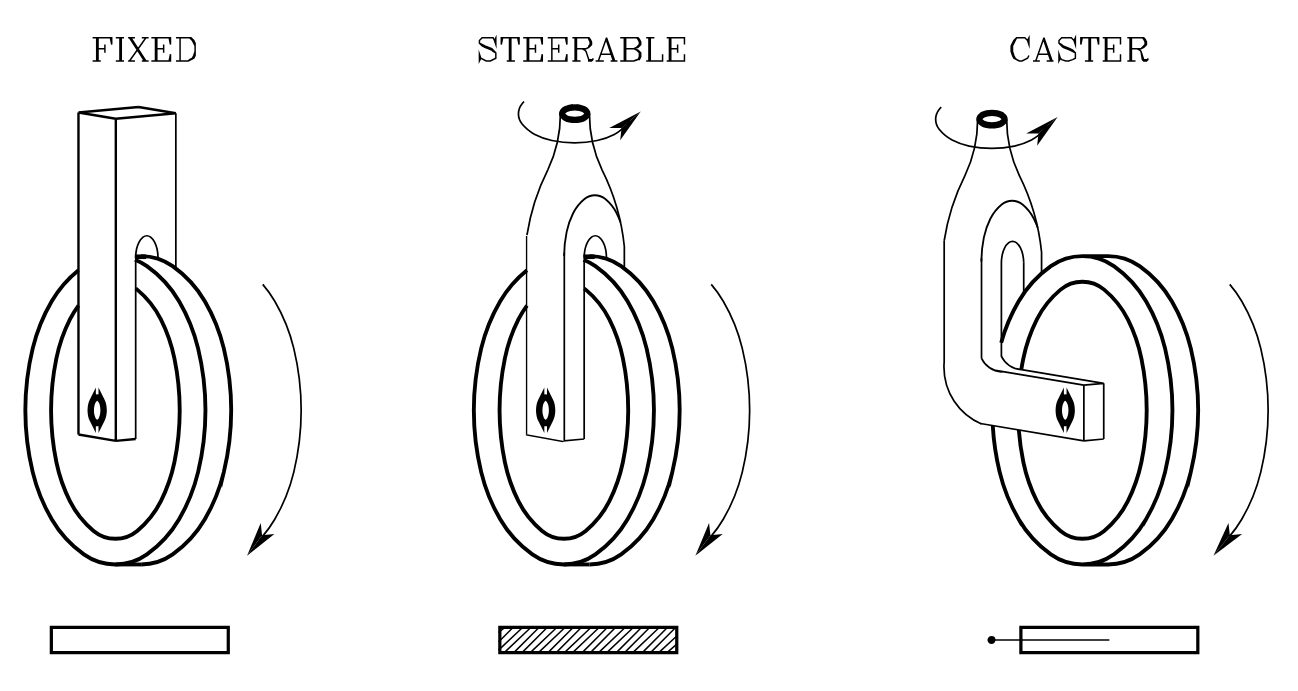
\includegraphics[width=150mm, keepaspectratio]{figures/021_wheels.png}
    \caption{Kerék mechanizmusok \cite{siciliano2010robotics}}
    \label{fig:wheels}
\end{figure}

\begin{itemize}
    \item \emph{Fix kerekek (fixed)}: csak irányban forognak (előre-hátra), nem képesek elfordulni oldalirányban. Általában meghajtott kerekek tartoznak ide, amelyek a robot hajtását biztosítják, például egy autó hátsó tengelyére szerelt kerekek. A robot bázisához mereven csatlakoznak és saját tengelyük körül forognak, amely ortogonális a kerék síkjára.\cite{siciliano2010robotics}
    \item \emph{Kormányozható (steerable) kerekek}: oldalirányban elfordíthatók, a haladási irányuk megváltoztatható, például autó első tengelyén lévő kerekek. A robot bázisához egy csuklóval csatlakoznak, mely lehetővé teszi a kerekek elfordulását, illetve erre merőleges saját tengellyel rendelkeznek (szintén merőleges a kerék síkjára), melyek körül forognak.\cite{siciliano2010robotics}
    \item \emph{Szabadonfutó (bolygó/caster) kerekek}: hasonló mechanikai csatlakozással rendelkeznek, mint az irányítható kerekek, azonban a robot bázisához való csatlakozásuknál található tengely körül szabadon fordulnak el, például irodai székek vagy bevásárló kocsi kerekei. A vertikális tengely nem metszi a kerék elfordulási tengelyét hanem egy "offset" távolságra helyezkedik el. Ezek a kerekek mechanikai stabilitásban segítik a robot bázist.\cite{siciliano2010robotics}
\end{itemize}

\subsection{Mobil kerekes robotok kinematikai modellje}
Kétféle csoportosítás különíthető el: holonomikus (nem tud mozogni a sík bármelyik irányában) és omnidirekcionális (tetszőleges irányba képes mozogni). Omnidirekcionális robotok mecanum (másik nevén svéd) kerekekkel (\refstruc{fig:023_omni_wheel}) felszerelt robotok, melyek több forgó alkatrésszel rendelkeznek, a kerék kerületen mentén független elfordulni képes görgők vannak amik segítségével oldalazó mozgást is végezhet a kerék tengelyével párhuzamosan. \cite{siciliano2010robotics} \cite{ros2_control_docs}

\begin{figure}[!ht]
    \centering
    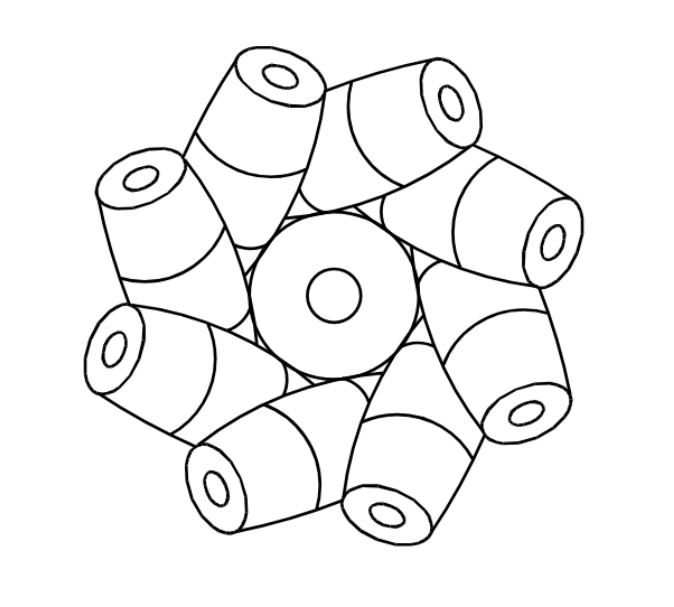
\includegraphics[width=75mm, keepaspectratio]{figures/023_omni_wheel.png}
    \caption{Mecanum kerék \cite{siciliano2010robotics}}
    \label{fig:023_omni_wheel}
\end{figure}

A dolgozatban vizsgált robotmodellek holonomikusak. Több fajta (előző pontban tárgyalt) kerék elrendezéssel hozható létre ilyen robotmodell. Klasszikusan a tricikli modell (\refstruc{fig:024_tricikli_car}), amely egy tengelyen két együttesen meghajtott kerékkel rendelkezik és egy kormányzott kerékkel. Az autókhoz hasonló modellek négy kerékkel (\refstruc{fig:024_tricikli_car}) ahol ebből kettő meghajtott és kettő kormányozható, vagy kettő egyszerre kormányozható és meghajtott plusz kettő stabilitásban asszisztáló fix kerékkel. Differenciál hajtású mobil robotok (\refstruc{fig:025_diff_model}) is a holonomikus robotok közé tartoznak, melyek két függetlenül meghajtott kerékkel és egy vagy több szabadon elforduló kerékkel szerelnek fel.  \cite{siciliano2010robotics} \cite{ros2_control_docs}

\begin{figure}[!ht]
    \centering
    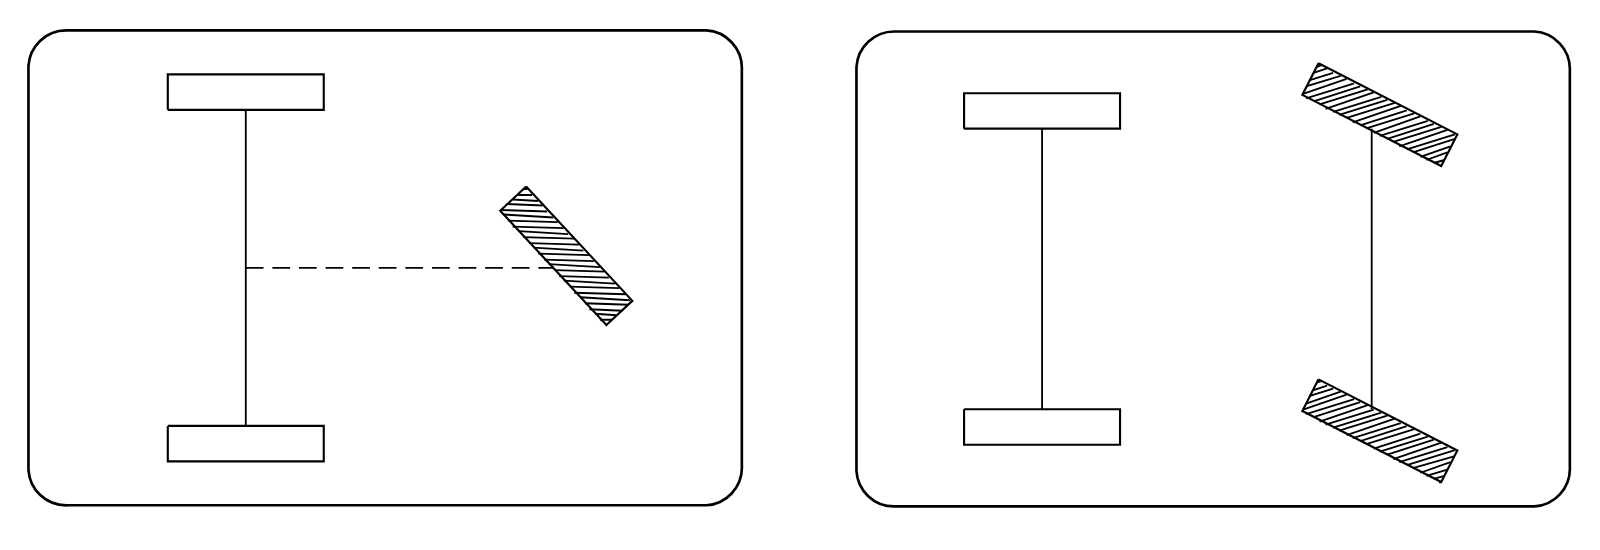
\includegraphics[width=150mm, keepaspectratio]{figures/024_tricikli_car.png}
    \caption{Tricikli és autó modellek \cite{siciliano2010robotics}}
    \label{fig:024_tricikli_car}
\end{figure}

\subsection{Differenciál hajtású robotok}
A diplomamunka során használt robotok közül mindegyik ebbe a kategóriába esik. Két szeparáltan meghajtott kerekének köszönhetően egyhelyeben képes megfordulni. A forgás tengelye a két kerék tengelyének közzéppontja. A passzív caster kerék vagy kerekek a stabilitásban segítenek, ezek lekövetik a robot mozgását. Ugye egy sík három pontból már felírható ezért a robot statikai egyensúlya nem jelent problémát, amíg a tömegközéppont vetülete a három vagy több kerek talajal való találkozási pontjainak egyenes szakaszokkal összekötő polinom belsejében marad. Mint mobil robot a differenciál hajtású szerkezetek munkatere virtuálisan végtelen, ha a munkateret a környezet egy altereként értelmezzük. A valóságban természetesen előjönnek olyan korlátok, mint a robot fizikai kiterjedése és a környezetben lévő akadályok relatív mérete és pozíciója. Természetesen itt sík felületet feltételezve (és kizárva lépcsőket, lifteket stb.) Mint nem omnidirekcionális robotmodell a lokális elmozdulására esnek korlátok. Nem tud rögtön a hajtott kerekek tengelyére merőleges irányába elmozdulni, ehhez szükséges fordulnia. De képesnek tekinthető bármely pozíciót felvenni csak nem rögtön. Ez úgy is kifejezhető, hogy a robot szabadsági fokainak száma alacsonyabb, mint a pozíciót leíró vektor változói. \cite{siciliano2010robotics} \cite{ros2_control_docs}

\begin{figure}[!ht]
    \centering
    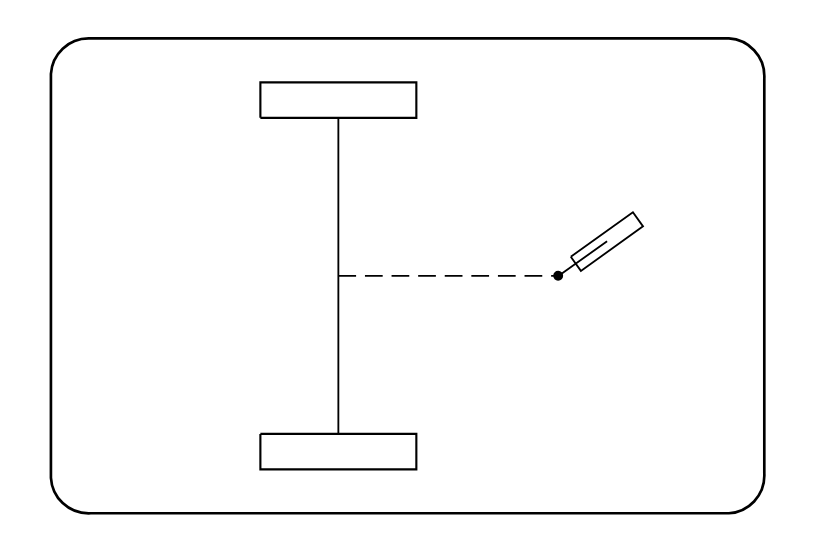
\includegraphics[width=75mm, keepaspectratio]{figures/025_diff_model.png}
    \caption{Differenciál hajtású robot modell \cite{siciliano2010robotics}}
    \label{fig:025_diff_model}
\end{figure}

TODO: előnyök, hátrányok más robotmechanizmusokkal szemben \\
TODO: turtlebot példa (kép)

Mozgásegyenletei felírásakor egyszerűsítve a modellt a bolygó kereket elhagyva.

\begin{figure}[!ht]
    \centering
    \includesvg[scale=1.2]{figures/022_diff_drive.svg}
    \caption{Differenciál hajtású robot 2 dimenzióban \cite{ros2_control_docs}}
    \label{fig:022_diff_drive}
\end{figure}

\begin{align}
    v_{b,x}      & = \frac{v_{right} + v_{left}}{2}, \\
    \omega_{b,z} & = \frac{v_{right} - v_{left}}{w},
\end{align}

\begin{align}
    v_{left}  & = v_{b,x} - \omega_{b,z} w / 2, \\
    v_{right} & = v_{b,x} + \omega_{b,z} w / 2,
\end{align}
